%TC:group tabular 1 1
\chapter{Results and Conclusions}

%This section should discuss issues you encountered as you tried to implement your experiments. What were the results of running the experiments? What conclusions can you draw from these results?

%During the work, you might have found that elements of your experiments were unnecessary or overly complex; perhaps third party libraries were available that simplified some of the functions that you intended to implement. If things were easier in some areas, then how did you adapt your project to take account of your findings?

%It is more likely that things were more complex than you first thought. In particular, were there any problems or difficulties that you found during implementation that you had to address? Did such problems simply delay you or were they more significant?

%If you had multiple experiments to run, it may be sensible to discuss each experiment in separate sections.
\section{Results}

This section will discuss both the alignment and run-time results. Whilst accuracy was extremely important in this project, a quick run-time would further increase the usability of the application, and therefore must be taken into consideration.

\subsection{Alignment results}
\label{ssec:align}

\begin{figure}[H]
  \centering
  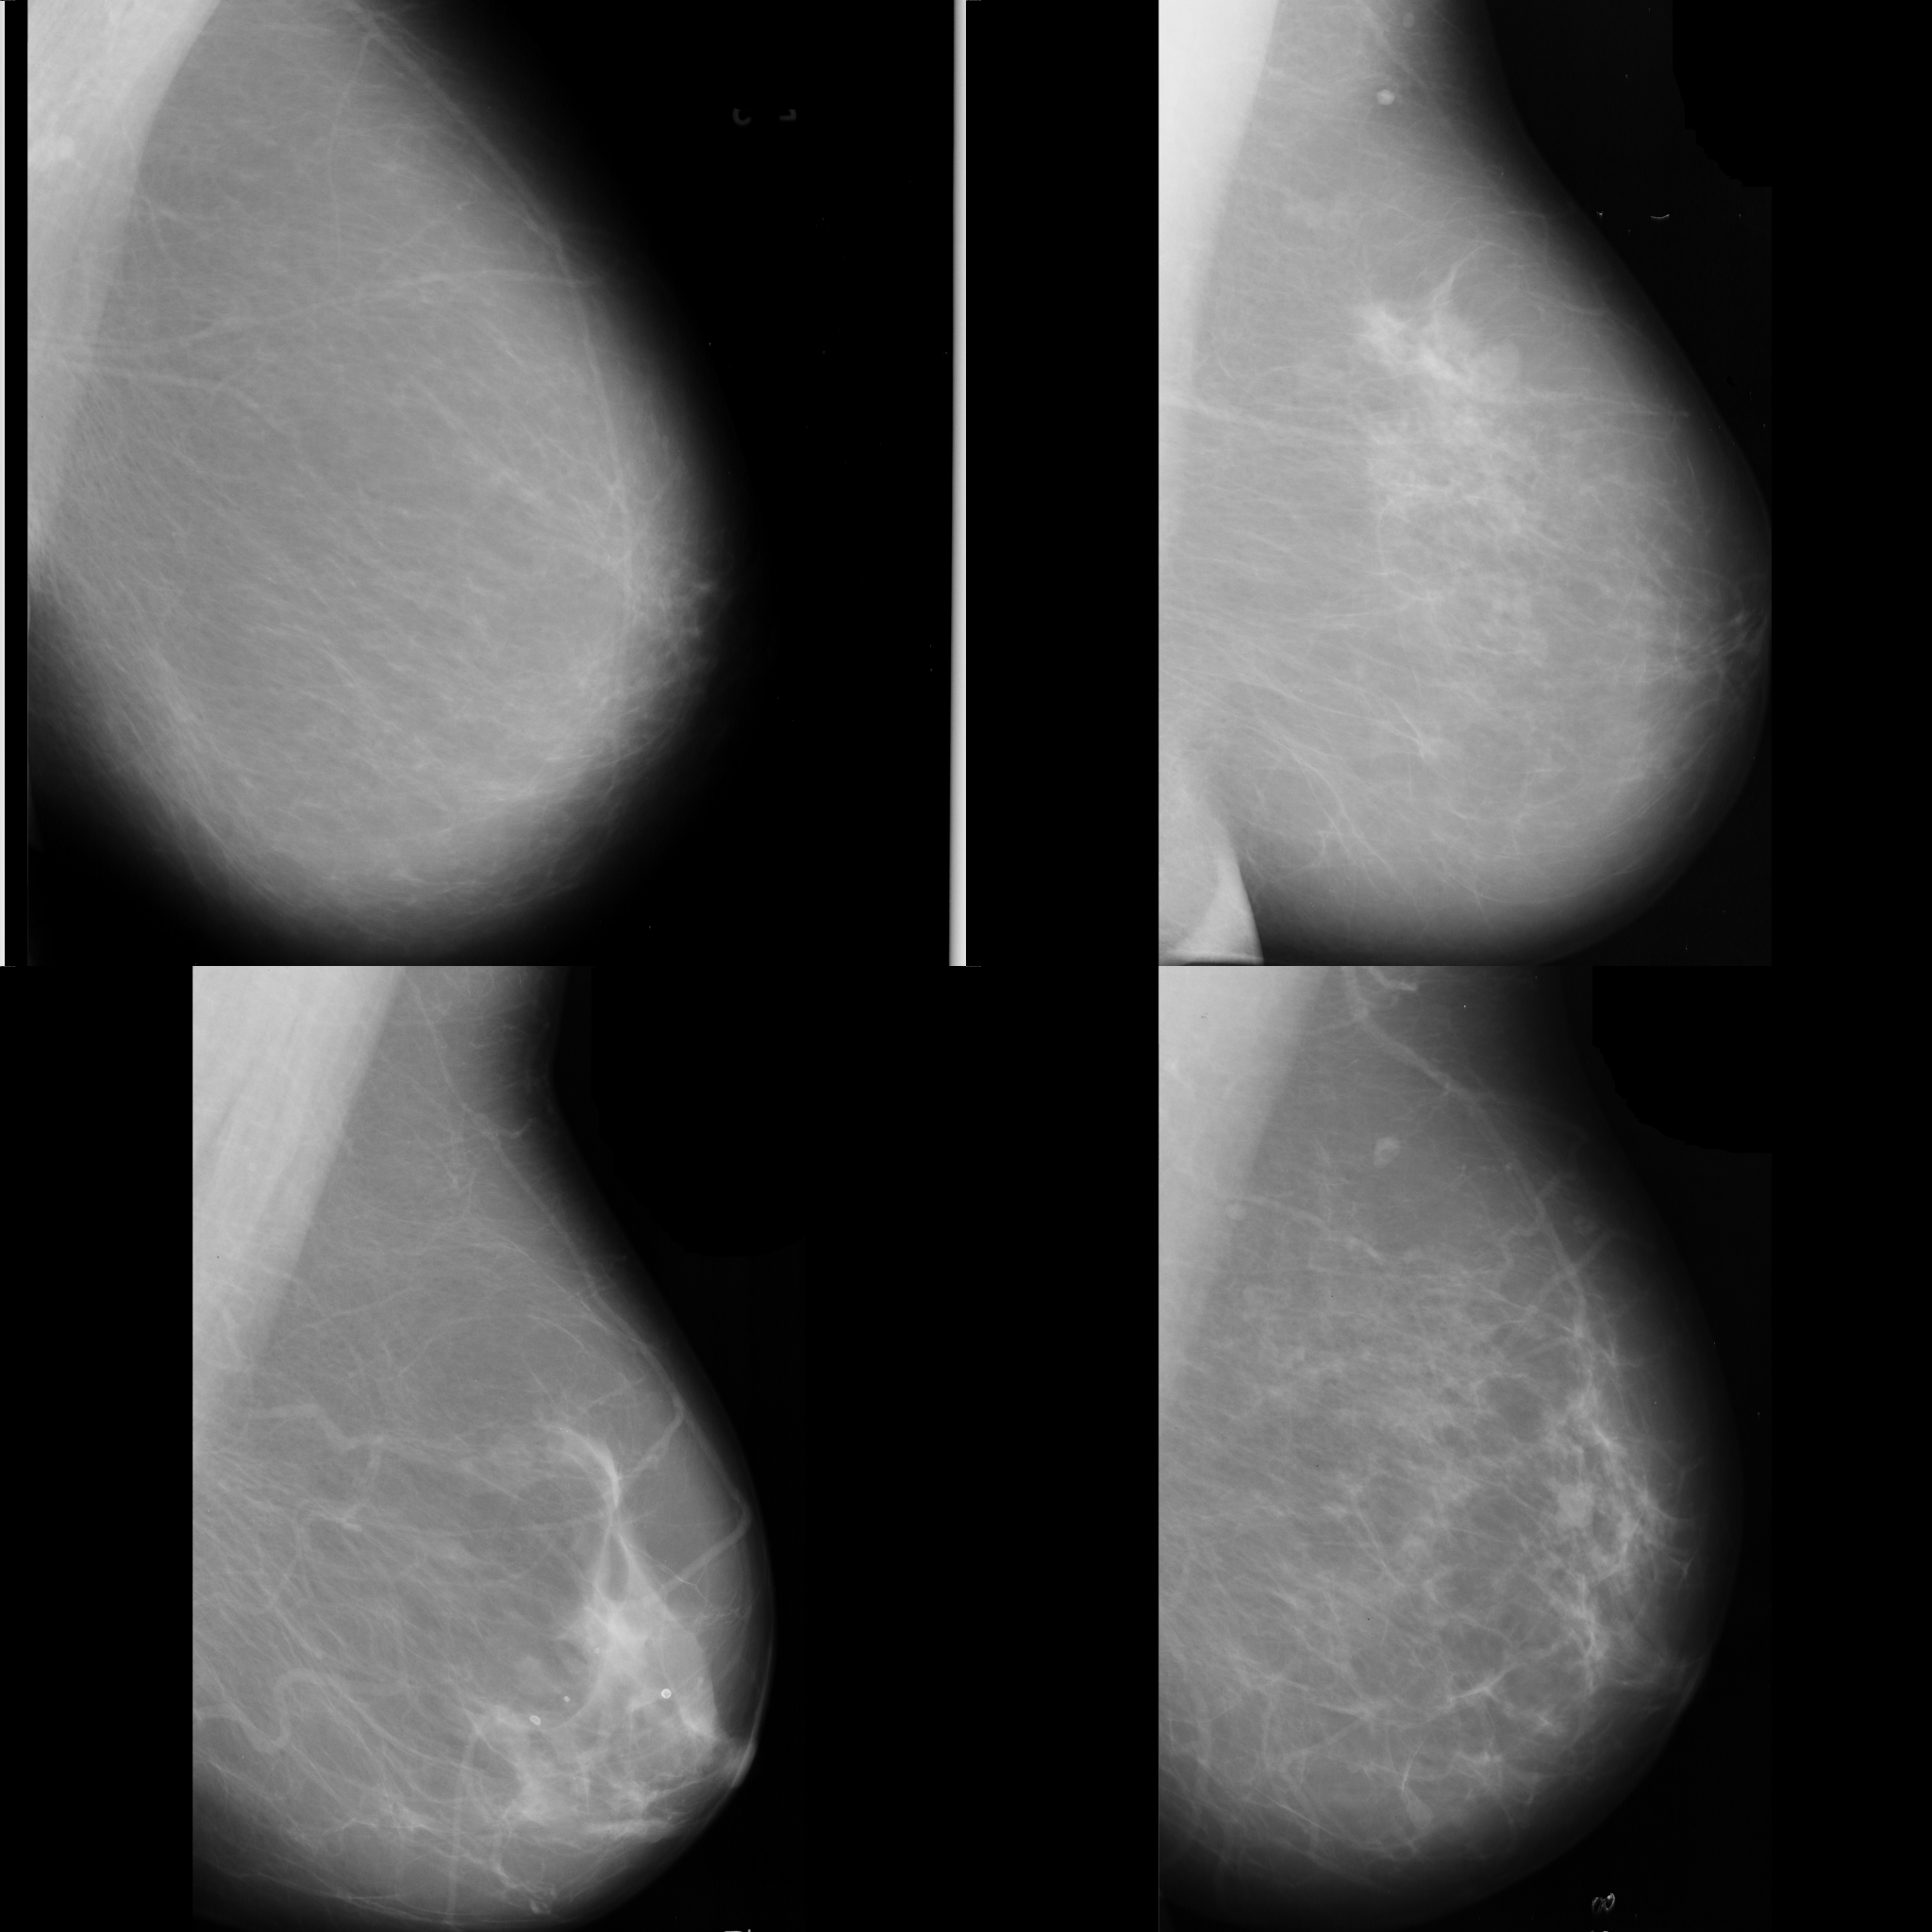
\includegraphics[width=0.4\textwidth]{Chapter3/results-img/big_scan.png}
  \caption{Four input scans.}
  \label{fig:input-data}
\end{figure}

Figure \ref{fig:input-data} shows the input image utilised in Figure \ref{fig:set1-results-all}. This large file contains four scans from the BI-RADS I classifcation, containing no masses in the tissue. Whilst relatively similar in size and shape, the tissue composition inside the breast is varied.

\begin{table}[H]
  \centering
  \begin{tabular}{|c|c|c|c|}
    \hline
      \textbf{Set No.} & \textbf{BI-RADS Class} & \textbf{No. of images} & \textbf{Pixel dimensions} \\ \hline
      1 & BI-RADS I & 4 & 2048 x 2048 \\ \hline
      2 & BI-RADS II & 6 & 3072 x 3972 \\ \hline
      3 & BI-RADS III & 8 & 3072 x 3072 \\ \hline
      4 & BI-RADS IV & 5 & 3072 x 3072 \\ \hline
  \end{tabular}
  \caption{Input image information.}
  \label{table:image-info}
\end{table}

Results for each set outlined in Table \ref{table:image-info} can be found in Appendix \ref{appendix:results}.

% http://tex.stackexchange.com/questions/202072/scale-y-and-x-axis-in-pgfplots
\begin{figure}[H]
  \begin{center}
  %  \iffalse
    \begin{tikzpicture}
      \begin{axis}[
        width=15cm,
        axis lines = middle,
        scaled ticks=false,
        grid=both,
        ymin=0,ymax=0.7,
        xlabel=$x$,ylabel=$y$,
        ytick={0,0.1,...,1},
        xtick={0,...,20},
        xlabel={\large Iteration},
        ylabel={\large Entropy},
        legend entries={Hybrid entropy,Non-Probabilistic entropy,Shannon entropy},
         x label style={at={(axis description cs:0.5,-0.05)},anchor=north},
         y label style={at={(axis description cs:-0.05,.5)},rotate=90,anchor=south},
        ]
        \addplot table [x=Iteration, y=Entropy, col sep=comma] {Chapter3/hybrid-img/hybrid20.csv};
      \addplot table [x=Iteration, y=Entropy, col sep=comma] {Chapter3/nonProb-img/nonprob20.csv};
      \addplot table [x=Iteration, y=Entropy, col sep=comma] {Chapter3/shannon-img/shannon-20.csv};
    \end{axis}
    \end{tikzpicture}
    %\fi
    \caption{Comparison of the reduction in entropy on each iteration on Sample Set 1.}
    \label{fig:set1-results-all}
  \end{center}
\end{figure}

Whilst the entropy decline of Shannon entropy and the fuzzy entropy algorithms can be plotted on one graph to show the general trend of decreasing entropy, it is worth noting that they are indeed not comparitive. As Shannon entropy does not contain any possibilistic uncertainty, the entropy outcome is vastly different in its calculation to that of both Non-Probabilistic and Hybrid.

\newpage
\subsubsection{Shannon Entropy}

\begin{figure}[H]
    \centering
    \begin{subfigure}[t]{0.3\textwidth}
        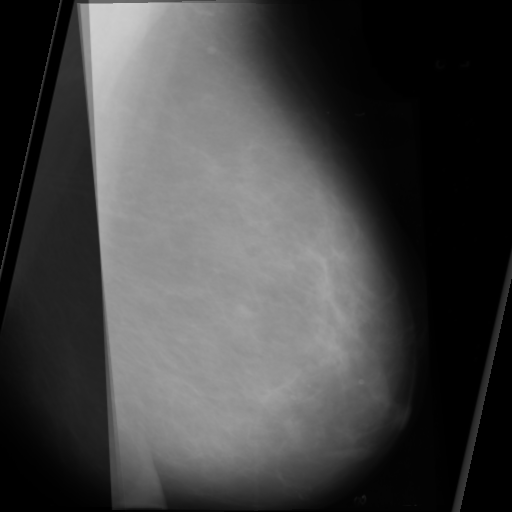
\includegraphics[width=\textwidth]{Chapter3/shannon-img/s-5-final.png}
        \caption{5 Shannon Entropy iterations on BI-RADS I sample set.}
        \label{fig:5-shannon}
    \end{subfigure} \hfill
    ~ %add desired spacing between images, e. g. ~, \quad, \qquad, \hfill etc.
      %(or a blank line to force the subfigure onto a new line)
    \begin{subfigure}[t]{0.3\textwidth}
        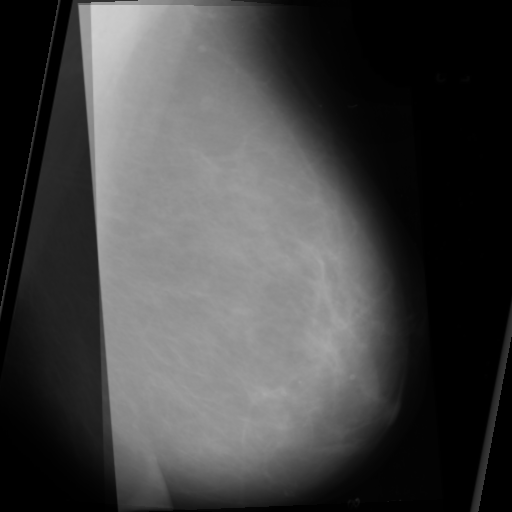
\includegraphics[width=\textwidth]{Chapter3/shannon-img/s-10-final.png}
        \caption{10 Shannon Entropy iterations on BI-RADS I sample set.}
        \label{fig:10-shannon}
    \end{subfigure} \hfill
    \begin{subfigure}[t]{0.3\textwidth}
      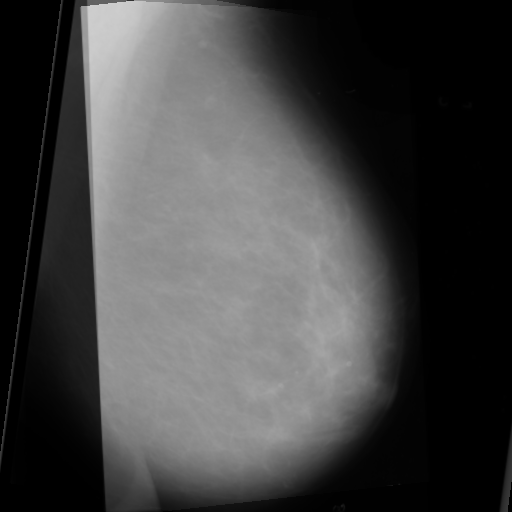
\includegraphics[width=\textwidth]{Chapter3/shannon-img/shannon-20.png}
      \caption{20 Shannon Entropy iterations on BI-RADS I sample set.}
      \label{fig:20-shannon}
    \end{subfigure}
\end{figure}

\begin{figure}[H]
  \begin{center}
  %  \iffalse
    \begin{tikzpicture}
      \begin{axis}[
        width=15cm,
        axis lines = middle,
        scaled ticks=false,
        grid=both,
        ymin=0,ymax=0.7,
        ytick={0,0.1,...,1},
        xtick={0,...,20},
        xlabel={\large Iteration},
        ylabel={\large Entropy},
        legend entries={Set 1: BI-RADS I,Set 2: BI-RADS II,Set 3: BI-RADS III, Set 4: BI-RADS IV},
         x label style={at={(axis description cs:0.5,-0.05)},anchor=north},
         y label style={at={(axis description cs:-0.05,.5)},rotate=90,anchor=south},
        ]
      \addplot table [x=Iteration, y=Entropy, col sep=comma] {Chapter3/shannon-img/shannon-20.csv};
      \addplot table [x=Iteration, y=Entropy, col sep=comma] {Appendix5/sample2/shannon/shannon_entropy.csv};
      \addplot table [x=Iteration, y=Entropy, col sep=comma] {Appendix5/sample3/shannon/shannon.csv};
      \addplot table [x=Iteration, y=Entropy, col sep=comma] {Appendix5/sample4/shannon/shannon.csv};
    \end{axis}
    \end{tikzpicture}
    %\fi
    \caption{Shannon: Comparison of the reduction in entropy from each Sample set, as summarised in Table \ref{table:shannon-entropy}.}
    \label{fig:shannon-graph}
  \end{center}
\end{figure}

\begin{table}[H]
  \centering
  \begin{tabular}{| c  c  c   c |}
    \textbf{Sample} & \textbf{Starting entropy} & \textbf{Final entropy} & \textbf{Entropy change} \\ \hline
    BI-RADS I & 0.416080 & 0.350700 & 0.06538 \\ \hline
    BI-RADS II & 0.574292 & 0.534195 & 0.040097 \\ \hline
    BI-RADS III & 0.363914 & 0.315340 & 0.048574 \\ \hline
    BI-RADS IV & 0.231113 & 0.210216 & 0.020897 \\
  \end{tabular}
  \caption{Shannon entropy difference table for each sample set.}
  \label{table:shannon-entropy}
\end{table}

The largest decrease in Shannon entropy over all four of the sample sets can be seen in BI-RADS I. The output for each of the sample sets is relatively sensible (as can be seen in  Appendix \ref{appendix:results} - Section \ref{sec:app-shannon}) and the run time of each iteration is quick due to the lookup table implementation (covered in later Subsection \ref{ssec:run-time}), demonstrating that Learned-Miller`s original code is still useful even upon mammograms.

The gradual straightening of the curve of all four sets, as represented in Figure \ref{fig:shannon-graph}, indicates a slowing in the reduction of entropy, which would most likely result in the over-congealment of the input images. Over-congealing is when the entropy is reduced to such a point that any further iterations could either: increase the entropy, or reduce the entropy to an unreasonable level.

\newpage
\subsubsection{Non-Probabilistic Entropy}

\begin{figure}[H]
    \centering
    \begin{subfigure}[t]{0.3\textwidth}
        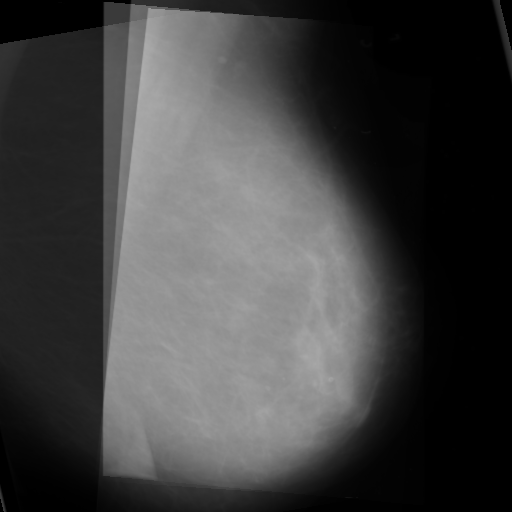
\includegraphics[width=\textwidth]{Chapter3/nonProb-img/nonProb-5.png}
        \caption{5 Non-Probabilistic entropy iterations on BI-RADS I sample set.}
        \label{fig:5-nonProb}
    \end{subfigure} \hfill
    ~ %add desired spacing between images, e. g. ~, \quad, \qquad, \hfill etc.
      %(or a blank line to force the subfigure onto a new line)
    \begin{subfigure}[t]{0.3\textwidth}
      \includegraphics[width=\textwidth]{Chapter3/nonProb-img/nonProb10.png}
        \caption{10 Non-Probabilistic entropy iterations on BI-RADS I sample set.}
        \label{fig:10-nonProb}
    \end{subfigure} \hfill
    \begin{subfigure}[t]{0.3\textwidth}
      \includegraphics[width=\textwidth]{Chapter3/nonProb-img/nonProb20.png}
      \caption{20 Non-Probabilistic entropy iterations on BI-RADS I sample set.}
      \label{fig:20-nonProb}
    \end{subfigure}
\end{figure}

\begin{figure}[H]
  \begin{center}
  %  \iffalse
    \begin{tikzpicture}
      \begin{axis}[
        width=15cm,
        axis lines = middle,
        scaled ticks=false,
        grid=both,
        ymin=0,ymax=0.05,
        ytick = {0, 0.01,...,0.05},
        yticklabel style={/pgf/number format/fixed,
                  /pgf/number format/precision=4},
        xtick={0,...,20},
        xlabel={\large Iteration},
        ylabel={\large Entropy},
        legend entries={Set 1: BI-RADS I,Set 2: BI-RADS II,Set 3: BI-RADS III, Set 4: BI-RADS IV},
         x label style={at={(axis description cs:0.5,-0.05)},anchor=north},
         y label style={at={(axis description cs:-0.1,.5)},rotate=90,anchor=south},
        ]
      \addplot table [x=Iteration, y=Entropy, col sep=comma] {Appendix5/sample1/nonProb/nonprob20.csv};
      \addplot table [x=Iteration, y=Entropy, col sep=comma] {Appendix5/sample2/nonProb/nonProb.csv};
      \addplot table [x=Iteration, y=Entropy, col sep=comma] {Appendix5/sample3/nonProb/nonProb.csv};
      \addplot table [x=Iteration, y=Entropy, col sep=comma] {Appendix5/sample4/nonProb/nonProb.csv};
    \end{axis}
    \end{tikzpicture}
    %\fi
    \caption{Non-Probabilistic: Comparison of the reduction in entropy over iterations, as in Table \ref{table:non-prob-entropy}.}
    \label{fig:non-prob-graph}
  \end{center}
\end{figure}

\begin{table}[H]
  \centering
  \begin{tabular}{| c | c | c  | c |}
    \textbf{Sample} & \textbf{Starting entropy} & \textbf{Final entropy} & \textbf{Entropy change} \\
    BI-RADS I & 0.015932 & 0.010889 & 0.005043 \\
    BI-RADS II & 0.024955 & 0.010888  & 0.014067 \\
    BI-RADS III & 0.028877 & 0.016796 & 0.012081 \\
    BI-RADS IV & 0.024644 & 0.006101  & 0.018543 \\
  \end{tabular}
  \caption{Entropy table for Non-Probabilistic}
  \label{table:non-prob-entropy}
\end{table}

As outlined in both Figure \ref{fig:non-prob-graph}, and Table \ref{table:non-prob-entropy}, the entropy for image alignment using the Non-Probabilistic algorithm tends to be quite low. Because of this, often the entropy decline seems to be quite low, however generally the intial entropy can be lower than the final entropy of Hybrid entropy.

Sample sets 1 \& 2 can be seen in Figure \ref{fig:non-prob-graph} to be fluctuating, especially in the latter iterations. This is due to over-congealing the image, as mentioned in the previous section. In Set 1 for example, the entropy of the images barely decreases between iterations four and twenty, therefore the algorithm could be stopped a lot quicker, saving time for the user.

\newpage
\subsubsection{Hybrid Entropy}
\label{sssec:hybrid-alignment}

\begin{figure}[H]
    \centering
    \begin{subfigure}[t]{0.3\textwidth}
        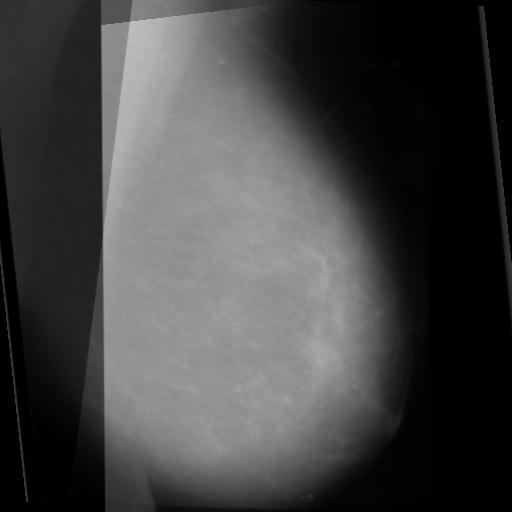
\includegraphics[width=\textwidth]{Chapter3/hybrid-img/hybrid-5.png}
        \caption{5 Hybrid entropy iterations on BI-RADS I sample set.}
        \label{fig:5-hybrid}
    \end{subfigure} \hfill
    ~ %add desired spacing between images, e. g. ~, \quad, \qquad, \hfill etc.
      %(or a blank line to force the subfigure onto a new line)
    \begin{subfigure}[t]{0.3\textwidth}
      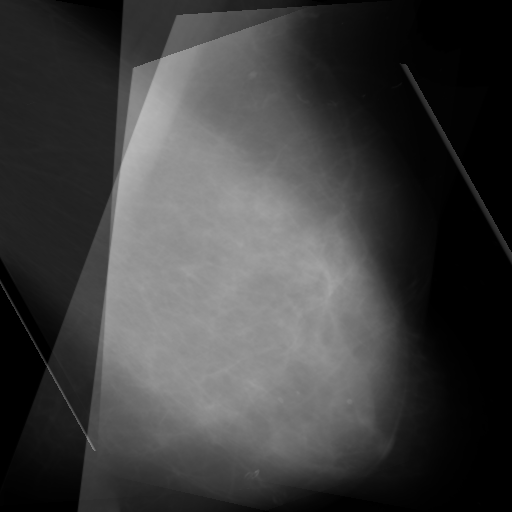
\includegraphics[width=\textwidth]{Chapter3/hybrid-img/hybrid-10.png}
        \caption{10 Hybrid entropy iterations on BI-RADS I sample set.}
        \label{fig:10-hybrid}
    \end{subfigure} \hfill
    \begin{subfigure}[t]{0.3\textwidth}
      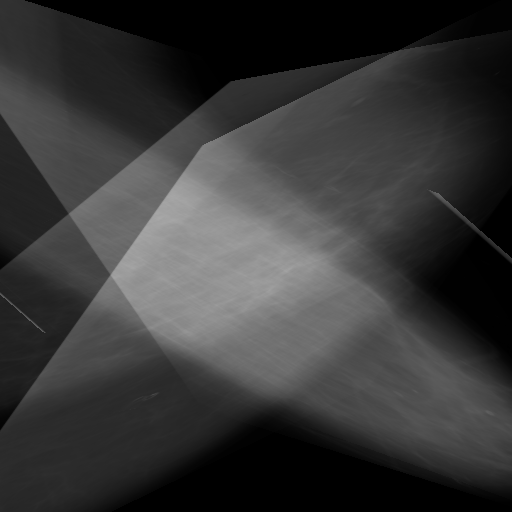
\includegraphics[width=\textwidth]{Chapter3/hybrid-img/hybrid20.png}
      \caption{20 Hybrid entropy iterations on BI-RADS I sample set.}
      \label{fig:20-hybrid}
    \end{subfigure}
\end{figure}

\begin{figure}[H]
  \begin{center}
  %  \iffalse
    \begin{tikzpicture}
      \begin{axis}[
        width=15cm,
        axis lines = middle,
        scaled ticks=false,
        grid=both,
        ymin=0,ymax=0.3,
        ytick = {0, 0.05,...,0.3},
        yticklabel style={/pgf/number format/fixed,
                  /pgf/number format/precision=3},
        xtick={0,...,20},
        xlabel={\large Iteration},
        ylabel={\large Entropy},
        legend entries={Set 1: BI-RADS I,Set 2: BI-RADS II,Set 3: BI-RADS III, Set 4: BI-RADS IV},
         x label style={at={(axis description cs:0.5,-0.05)},anchor=north},
         y label style={at={(axis description cs:-0.1,.5)},rotate=90,anchor=south},
        ]
      \addplot table [x=Iteration, y=Entropy, col sep=comma] {Appendix5/sample1/hybrid/hybrid20.csv};
      \addplot table [x=Iteration, y=Entropy, col sep=comma] {Appendix5/sample2/hybrid/hybrid.csv};
      \addplot table [x=Iteration, y=Entropy, col sep=comma] {Appendix5/sample3/hybrid/hybrid.csv};
      \addplot table [x=Iteration, y=Entropy, col sep=comma] {Appendix5/sample4/hybrid/hybrid.csv};
    \end{axis}
    \end{tikzpicture}
    %\fi
    \caption{Hybrid: Comparison of the reduction in entropy over iterations, as in Table \ref{table:hybrid-entropy}.}
  \end{center}
\end{figure}

\begin{table}[H]
  \centering
  \begin{tabular}{| c | c | c  | c |}
    \textbf{Sample} & \textbf{Starting entropy} & \textbf{Final entropy} & \textbf{Entropy change} \\
    BI-RADS I & 0.193522 & 0.051228 & 0.142294 \\
    BI-RADS II & 0.089658 & 0.021976  & 0.067682 \\
    BI-RADS III & 0.093583 & 0.027946 & 0.065637 \\
    BI-RADS IV & 0.062255 & 0.022408  & 0.039847 \\
  \end{tabular}
  \caption{Entropy table for Hybrid}
  \label{table:hybrid-entropy}
\end{table}

In the previous two sections, over-congealing has been spoken about. Figure \ref{fig:20-hybrid} is a perfect example of an image becoming overly-congealed. However, the graph does not seem to mimic the erratic behavior displayed by Non-Probabilistic entropy. This brings to light how different the fuzzy entropy implementations can be, and how the non-deterministic nature of the \Gls{Congealing} algorithm can lead to dramatically different results, depending upon which order the image transformations are run.

It could be mistakenly understood that Hybrid entropy should be stopped between five and ten iterations, however it is purely dependent upon the dataset fed into the \Gls{Congealing} algorithm utilising Hybrid alignment, as is demonstrated in Figure \ref{fig:hybrid-behaviour}. Whilst Figure \ref{fig:hybrid-set3-5iters}, utilising the third data set (BI-RADS III,) could be seen to pass the optimal alignment at only five iterations, Figure \ref{fig:hybrid-set4-10iters}, utilising the fourth data set (BI-RADS IV) is nearing the best possible average. This is one reason it is difficult to ascertain when to terminate the \Gls{Congealing} algorithm automatically.

\begin{figure}[H]
    \centering
    \begin{subfigure}[t]{0.4\textwidth}
      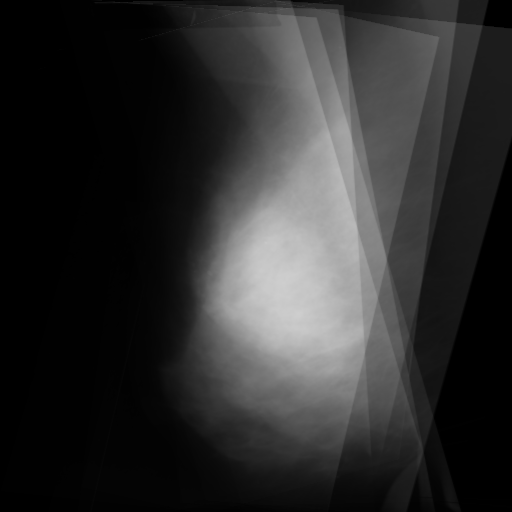
\includegraphics[width=\textwidth]{Appendix5/sample3/hybrid/5_hybrid.png}
        \caption{Sample set 3 (BI-RADS III) after 5 iterations.}
        \label{fig:hybrid-set3-5iters}
    \end{subfigure} \hfill
    \begin{subfigure}[t]{0.4\textwidth}
        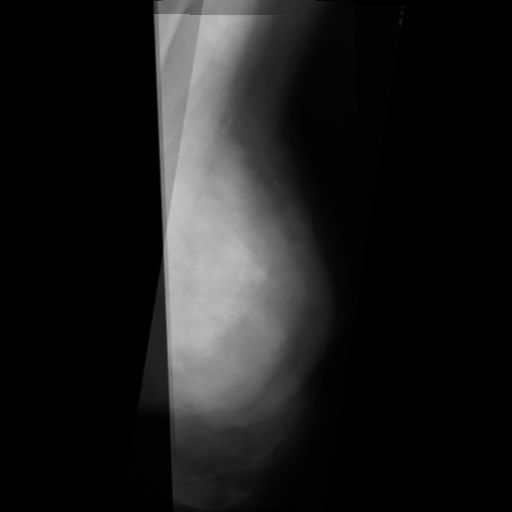
\includegraphics[width=\textwidth]{Appendix5/sample4/hybrid/hybrid_10.png}
        \caption{Sample set 4 (BI-RADS IV) after 10 iterations.}
        \label{fig:hybrid-set4-10iters}
    \end{subfigure}
    ~ %add desired spacing between images, e. g. ~, \quad, \qquad, \hfill etc.
      %(or a blank line to force the subfigure onto a new line)
      \caption{Example of how different datasets behave when aligning with Hybrid entropy.}
      \label{fig:hybrid-behaviour}
\end{figure}
